\chapter{Análise Bibliográfica sobre Processamento de Linguagem Natural, por Lucas de Almeida Bandeira Macedo}

\section{Planejamento do estudo}

Com a vinda de assistentes virtuais, como a Alexa (Amazon), Cortana (Microsoft) ou Siri (Apple), as pessoas costumam se perguntar cada vez mais: "como que esse programa está entendendo o que eu falo?".

Mas não só de assistentes virtuais vive o Processamento de Linguagem Natural (também conhecido como NLP - Natural Language Processing), afinal, qualquer texto ou fala pode ser interpretado por uma máquina e devidamente classificado. Por exemplo, uma aplicação famosa é o "classificador de sentimentos", em que um modelo treinado consegue classificar textos entre sentimentos "positivos" ou "negativos". Com a ascensão do Twitter, uma rede social baseada em pequenos textos de não mais que 280 caracteres, NLP se torna cada vez mais interessante.

Assim, as perguntas que traçam o norte para este estudo são:

\begin{itemize}
    \item Quais os principais conceitos ligados com Processamento de Linguagem Natural?
    \item Como se dá o progresso das pesquisas em NLP ao longo dos anos? As redes sociais influenciaram esse crescimento?
    \item Qual o estado da estrutura social da comunidade de NLP?
\end{itemize}

\subsection{Uso do Bibliometrix e Biblioshiny}

Será usada a ferramenta Bibliometrix, com sua função Biblioshiny, para gerar gráficos e grafos iterativos e personalizáveis, para auxiliar na interpretação da realidade científica do tópico.

\section{Coleta de dados}

A coleta de dados foi feita utilizando o site Web of Science (WoS), no dia 03/02/2022, através do portal periódico da capes.

A pesquisa foi realizada utilizando as edições "Science Citation Index Expanded" e "Conference Proceedings Citation Index – Science", ambas coleções são voltadas para, principalmente, as ciências exatas.

A \textit{string} (ou \textit{query}) de busca inicialmente utilizada foi a seguinte:

\lstinputlisting[numbers=left,basicstyle=\normalsize\ttfamily,caption={Query de busca sobre Procesasmento de Linguagem Natural.},label=queryNLP03022022]
{experiments/ABMHub/PesquisaBibliometrica/NLP/pesquisa_velha.txt}

\subsection{Explicação para os termos de busca usados}
\label{sec:ABMHub:query}

A proposta é apenas pesquisar sobre Processamento de Linguagem Natural, sem muito rigor na aplicação em que essa arquitetura de rede neural é aplicada. Portanto, inicialmente a pesquisa foi apenas "natural language processing".

Porém, uma rápida olhada pelos artigos retornados evidenciou uma grande quantidade de artigos sobre linguísticas, e áreas que não são da computação. Como o objetivo aqui adquirir modelos de Deep Learning, a pesquisa foi ajustada para filtrar apenas por NLP ligadas diretamente a computação e inteligência artificial, evidenciado pelas cláusulas "neural network", "(machine or deep) and learning" e "artificial intelligence". Essa nova pesquisa trouxe melhores resultados, todos evidenciando redes neurais e variadas técnicas de machine learning. O total de registros retornado pela query foi 10152, e esse dataset será, daqui para frente, mencionado como "\textit{NLP@LABM}".

\subsubsection{Refinamento da Coleta de Dados}
\label{sec:abmhub:refinamento}

 Em seguida, em uma análise mais fina, utilizando a \textbf{Rede de Co-ocorrências de Palavras-chave}, podemos evidenciar outras palavras chaves que estavam aparecendo entre os registros da pesquisa, que não deveriam estar aparecendo. É possível observar na imagem \ref{fig:ABMHub:NLPgraph1}, palavras como "câncer" ou "diagnóstico" que estão relacionadas a visão computacional mais que NLP, aparecendo com pesos não-desprezíveis.
 
 \begin{figure}
    \centering
    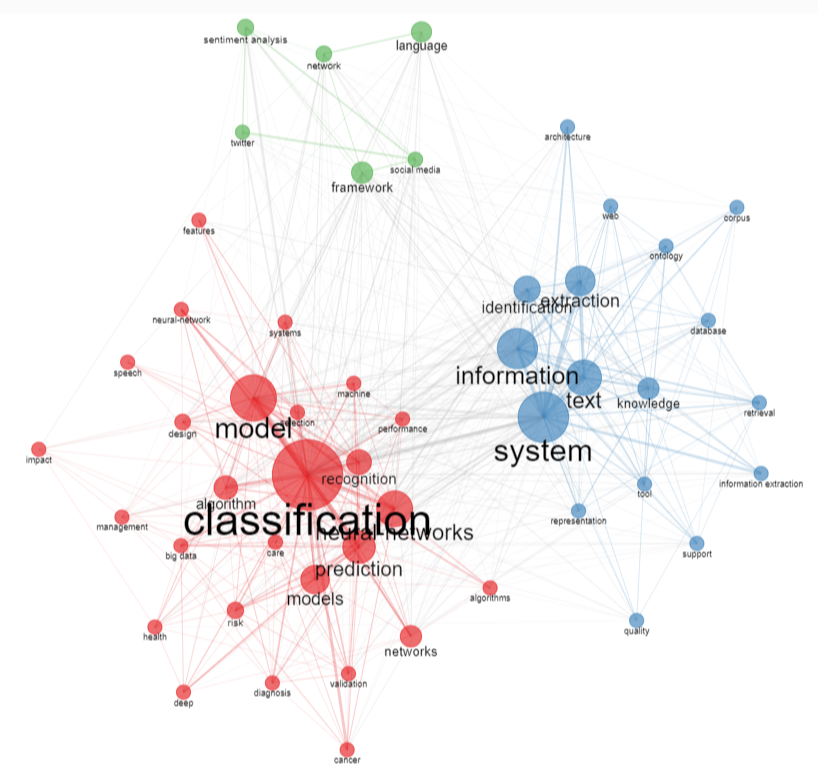
\includegraphics[width=1\textwidth]{experiments/ABMHub/PesquisaBibliometrica/NLP/grafo_keywords.png}
    \caption{Grafo de relação de keywords do dataset \textit{NLP@LABM}}
    \label{fig:ABMHub:NLPgraph1}
\end{figure}

Assim, é necessário uma nova iteração da pesquisa, para evitar que registros de visão computacional corrompam a pesquisa de NLP. É delicado fazer isso, pois existem muitas menções a Visão Computacional nos registros de LP, já que ambos são ligados a Deep Learning, então retirar a keyword "Visão Computacional" provavelmente removeria muitos registros que não gostaríamos de remover da pesquisa. Assim, a melhor solução encontrada foi remover palavras que não têm intersecção entre os dois assuntos. Por exemplo, "medical", "cancer" e "diagnosis".

Assim, chegamos na mais recente query:

\lstinputlisting[numbers=left,basicstyle=\normalsize\ttfamily,caption={Query refinada de busca sobre Processamento de Linguagem Natural.},label=queryRefinadaNLP03022022]
{experiments/ABMHub/PesquisaBibliometrica/NLP/pesquisa_nova.txt}

Esta query refinada retornou 8557 registros, e esse novo dataset, que será usado ao longo desse estudo, é nomeado de \textit{NLP2@LABM}.

\subsection{Filtragem de registros}

Após o refino, foi estabelecido que usaremos o dataset \textit{NLP2@LABM} de 8557 registros. Portanto, podemos começar a tratá-lo e analisá-lo. Para isso, começamos filtrando registros indesejados, como prévias de artigos, críticas sobre outros arquivos, cartas e etc. Assim, deixaremos apenas os artigos, pois é o método padrão de publicação científica, e capítulos de livros, já que é um tipo de publicação recorrente na área. Após o filtro, reduzimos nosso dataset para 3308 registros.

\subsection{Análise descritiva do \textit{dataset} \textit{NLP2@LABM}}

Ainda utilizando a ferramenta Bibliometrix, faremos uma análise descritiva do dataset adquirido, ou seja cálculos de diversas métricas para trazer \textit{insights}.

\begin{description}
    \item [\textit{Timespan}] De 1990 até 2022 (hoje). Não foram encontrados registros de 1945 até 1989.
    \item [\textit{Sources (Journals, Books, etc)}] 750 fontes diferentes de artigos.
    \item [\textit{Average years from publication}] A média do tempo de publicação dosartigos no dataset é de 3,85 anos.
    \item [\textit{Average citations per documents}] Cada artigo foi citado em média 14.03 vezes.
    \item [\textit{Average citations per year per doc}] Os artigos do dataset por inteiro são, em média, citados 2567 vezes por ano.
    \item [\textit{References}] Os artigos têm 108452 referência para outras fontes.
    \item [\textit{Keywords Plus (ID)}] Há 2414 diferentes palavras chaves.
    \item [\textit{Author's Keywords (DE)}] Há 7439 diferentes palavras chaves, segundo os autores.
    \item [\textit{Authors}] Há 10028 diferentes autores.
    \item [\textit{Author Appearances}] Há 13237 autores (considerando repetição nomes para diferentes artigos).
    \item [\textit{Authors of single-authored documents}] Há 154 autores que fizeram trabalhos sozinhos.
    \item [\textit{Authors of multi-authored documents}] Há 9874 autores que fizeram trabalhos com outras pessoas.
    \item [\textit{Single-authored documents}] Há 163 trabalhos com apenas um autor.
    \item [\textit{Documents per Author}] Há, em média, 0,33 autores por trabalho.
    \item [\textit{Authors per Document}] Há, em média, 3,03 trabalhos por autor.
    \item [\textit{Co-Authors per Documents}] As 13237 aparições de autores se distribuem, em média 4 vezes para os 3308 documentos do dataset.
    \item [\textit{Collaboration Index}] Os autores que editaram artigos com um ou mais co-autores, colaboraram em media 3,54 vezes para editar os elaborados em co-autoria.
\end{description}

\subsection{Evolução da Produção Científica}

A evolução da produção científica do assunto é um dos principais motivadores dessa pesquisa. Afinal, com a quantidade absurda de dados que existem hoje livremente disponíveis na internet (e em exponencial crescimento), provavelmente influencia muito a qualidade de modelos gerados em qualquer área de machine learning. É esperado que, motivado por essa crescente de dados, e com a popularização de assistentes virtuais, NLP seja um tópico cada vez mais estudado.

 \begin{figure}
    \centering
    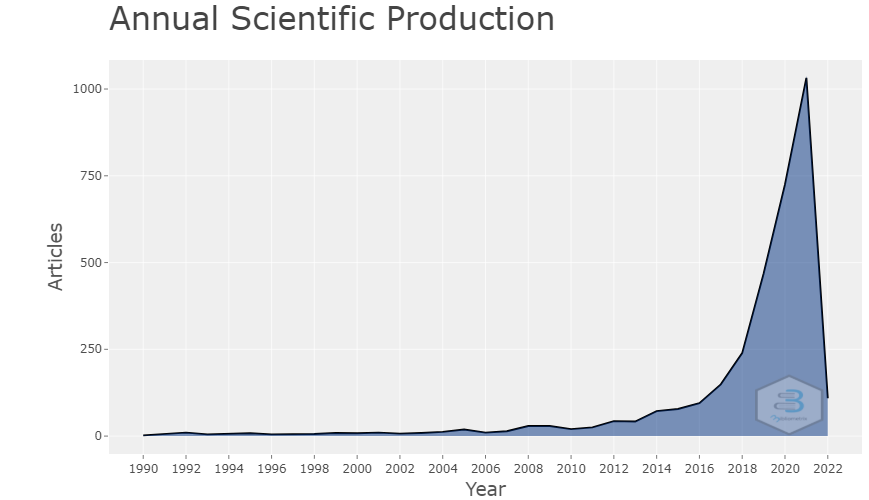
\includegraphics[width=1\textwidth]{experiments/ABMHub/PesquisaBibliometrica/NLP/anualScientificProduction.png}
    \caption{Produção científica anual sobre o \textit{dataset} \textit{NLP2@LABM}}
    \label{fig:ABMHub:ASP}
\end{figure}

Podemos ver que as suposições anteriores são verdadeiras (ou, ao menos, aparentemente verdadeiras). Como visto na figura \ref{fig:ABMHub:ASP}, a crescente absurda e exponencial em deep learning entre 2016 e 2021 realmente dá pistas que NLP está cada vez mais relevante no mundo moderno, e que continuará crescendo em influência por um bom tempo. É importante ressaltar que a queda apresentada no fim do gráfico ocorre apenas porque esses registros foram extraídos no começo do ano 2022.

Também é interessante observar que o primeiro registro é em 1990. O conceito de NLP foi inventado antes dessa data, mas apenas a partir desse ponto que NLP começou a ser estudado junto com Machine Learning, e a query utilizada (seção \ref{sec:ABMHub:query}) especifica que é necessária a ligação de processamento de linguagem natural com inteligência artificial.

\subsection{Evolução das Citações}

 \begin{figure}
    \centering
    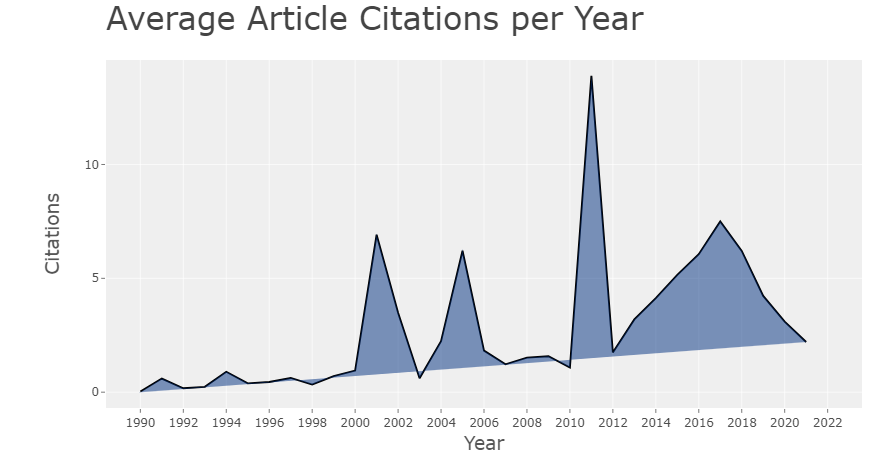
\includegraphics[width=1\textwidth]{experiments/ABMHub/PesquisaBibliometrica/NLP/citationsPerYear.png}
    \caption{Produção científica anual sobre o \textit{dataset} \textit{NLP2@LABM}}
    \label{fig:ABMHub:CPY}
\end{figure}

Podemos perceber que há um claro crescimento médio desde 1990 das citações médias por ano. Uma das coisas que mais chama atenção são os 4 picos no gráfico: em 2001, 2005, 2011 e 2017. Esses provavelmente são de artigos (ou grupos de artigos) que tiveram um impacto fora do comum, trazendo novos conceitos ou realizando descobertas fantásticas.

Esta é, inclusive, uma das perguntas feitas como motivação de pesquisa: "Como se dá o progresso das pesquisas em NLP ao longo dos anos? As redes sociais influenciaram esse crescimento?". Vemos que há crescimento mas, exclusivamente através desses dados, é difícil tirar conclusões sobre a relação deste crescimento com a vinda de redes sociais. 

\subsection{\textit{Three-Field Plots (Sankey diagram)}}

Como o nome indica, "Three-Field Plots" são tipos de gráficos que buscam correlacionar três tipos de dados diferentes, sem a necessidade de uma terceira dimensão adicionada em cima de um gráfico bidimensional. Na imagem \ref{fig:ABMHub:TFP}, temos um exemplo de plotagem de três campos que interliga os autores presentes no dataset, com fontes que eles citaram, assim como palavras chaves que costumam usar em seus artigos. 

 \begin{figure}
    \centering
    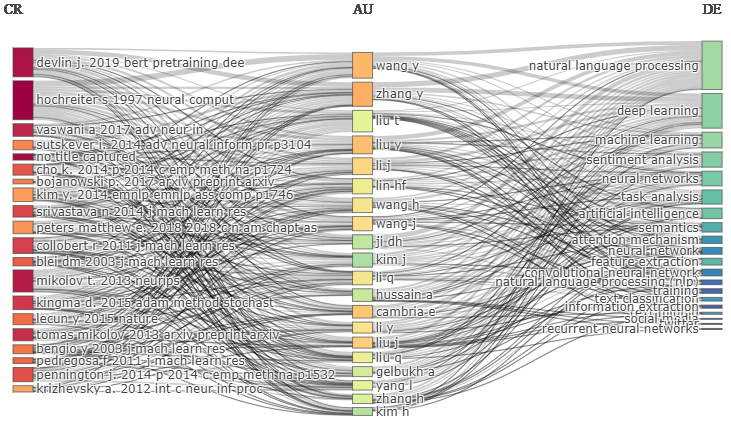
\includegraphics[width=1\textwidth]{experiments/ABMHub/PesquisaBibliometrica/NLP/tfp1.png}
    \caption{Three Field Plot - Citações, Autores e Palavras chaves}
    \label{fig:ABMHub:TFP1}
\end{figure}

Nessa plotagem, podemos extrair algumas informações muito interessantes sobre o estado atual de NLP. Primeiramente, vemos que o artigo mais citado por todos os artigos do dataset aqui apresentado é sobre computação neural (ou redes neurais), o que faz muito sentido, considerando que a NLP moderna é baseada em machine e deep learning. Outra observação interessante é que os artigos, em geral, são igualmente citados, mostrando que existe uma série de conceitos base para a NLP que são usados na maioria das aplicações do conceito.

Outro ponto interessante é que quase todos os autores listados no gráfico são chineses. Isso evidencia muito claramente a ascensão da China como potencia intelectual e tecnológica, principalmente em uma área tão relevante como a Inteligência Artificial.

Por último, as keywords também merecem sua atenção. Como esperado por ser o foco do dataset, Processamento de Linguagem Natural é a palavra-chave com mais menções. Mas, em seguida, vemos "Deep Learning", "Machine Learning" e "Neural Networks", o que faz muito sentido, partindo do princípio que (como dito anteriormente), NLP se apoia nesses conceitos atualmente. Também temos, com tamanho considerável, "sentiment analysis" e "task analysis", que são aplicações muito famosas de NLP.

\subsection{Análise da estrutura conceitual}

Nessa seção, analisaremos mais profundamente a estrutura conceitual do dataset \textit{NLP2@LABM}, afinal, essa é uma das perguntar norteadoras da pesquisa, então deve ser respondida com muita clareza. Essa análise ocorrerá pela análise de correspondência de keywords, parecido com a análise presente na seção \ref{sec:abmhub:refinamento}.

 \begin{figure}
    \centering
    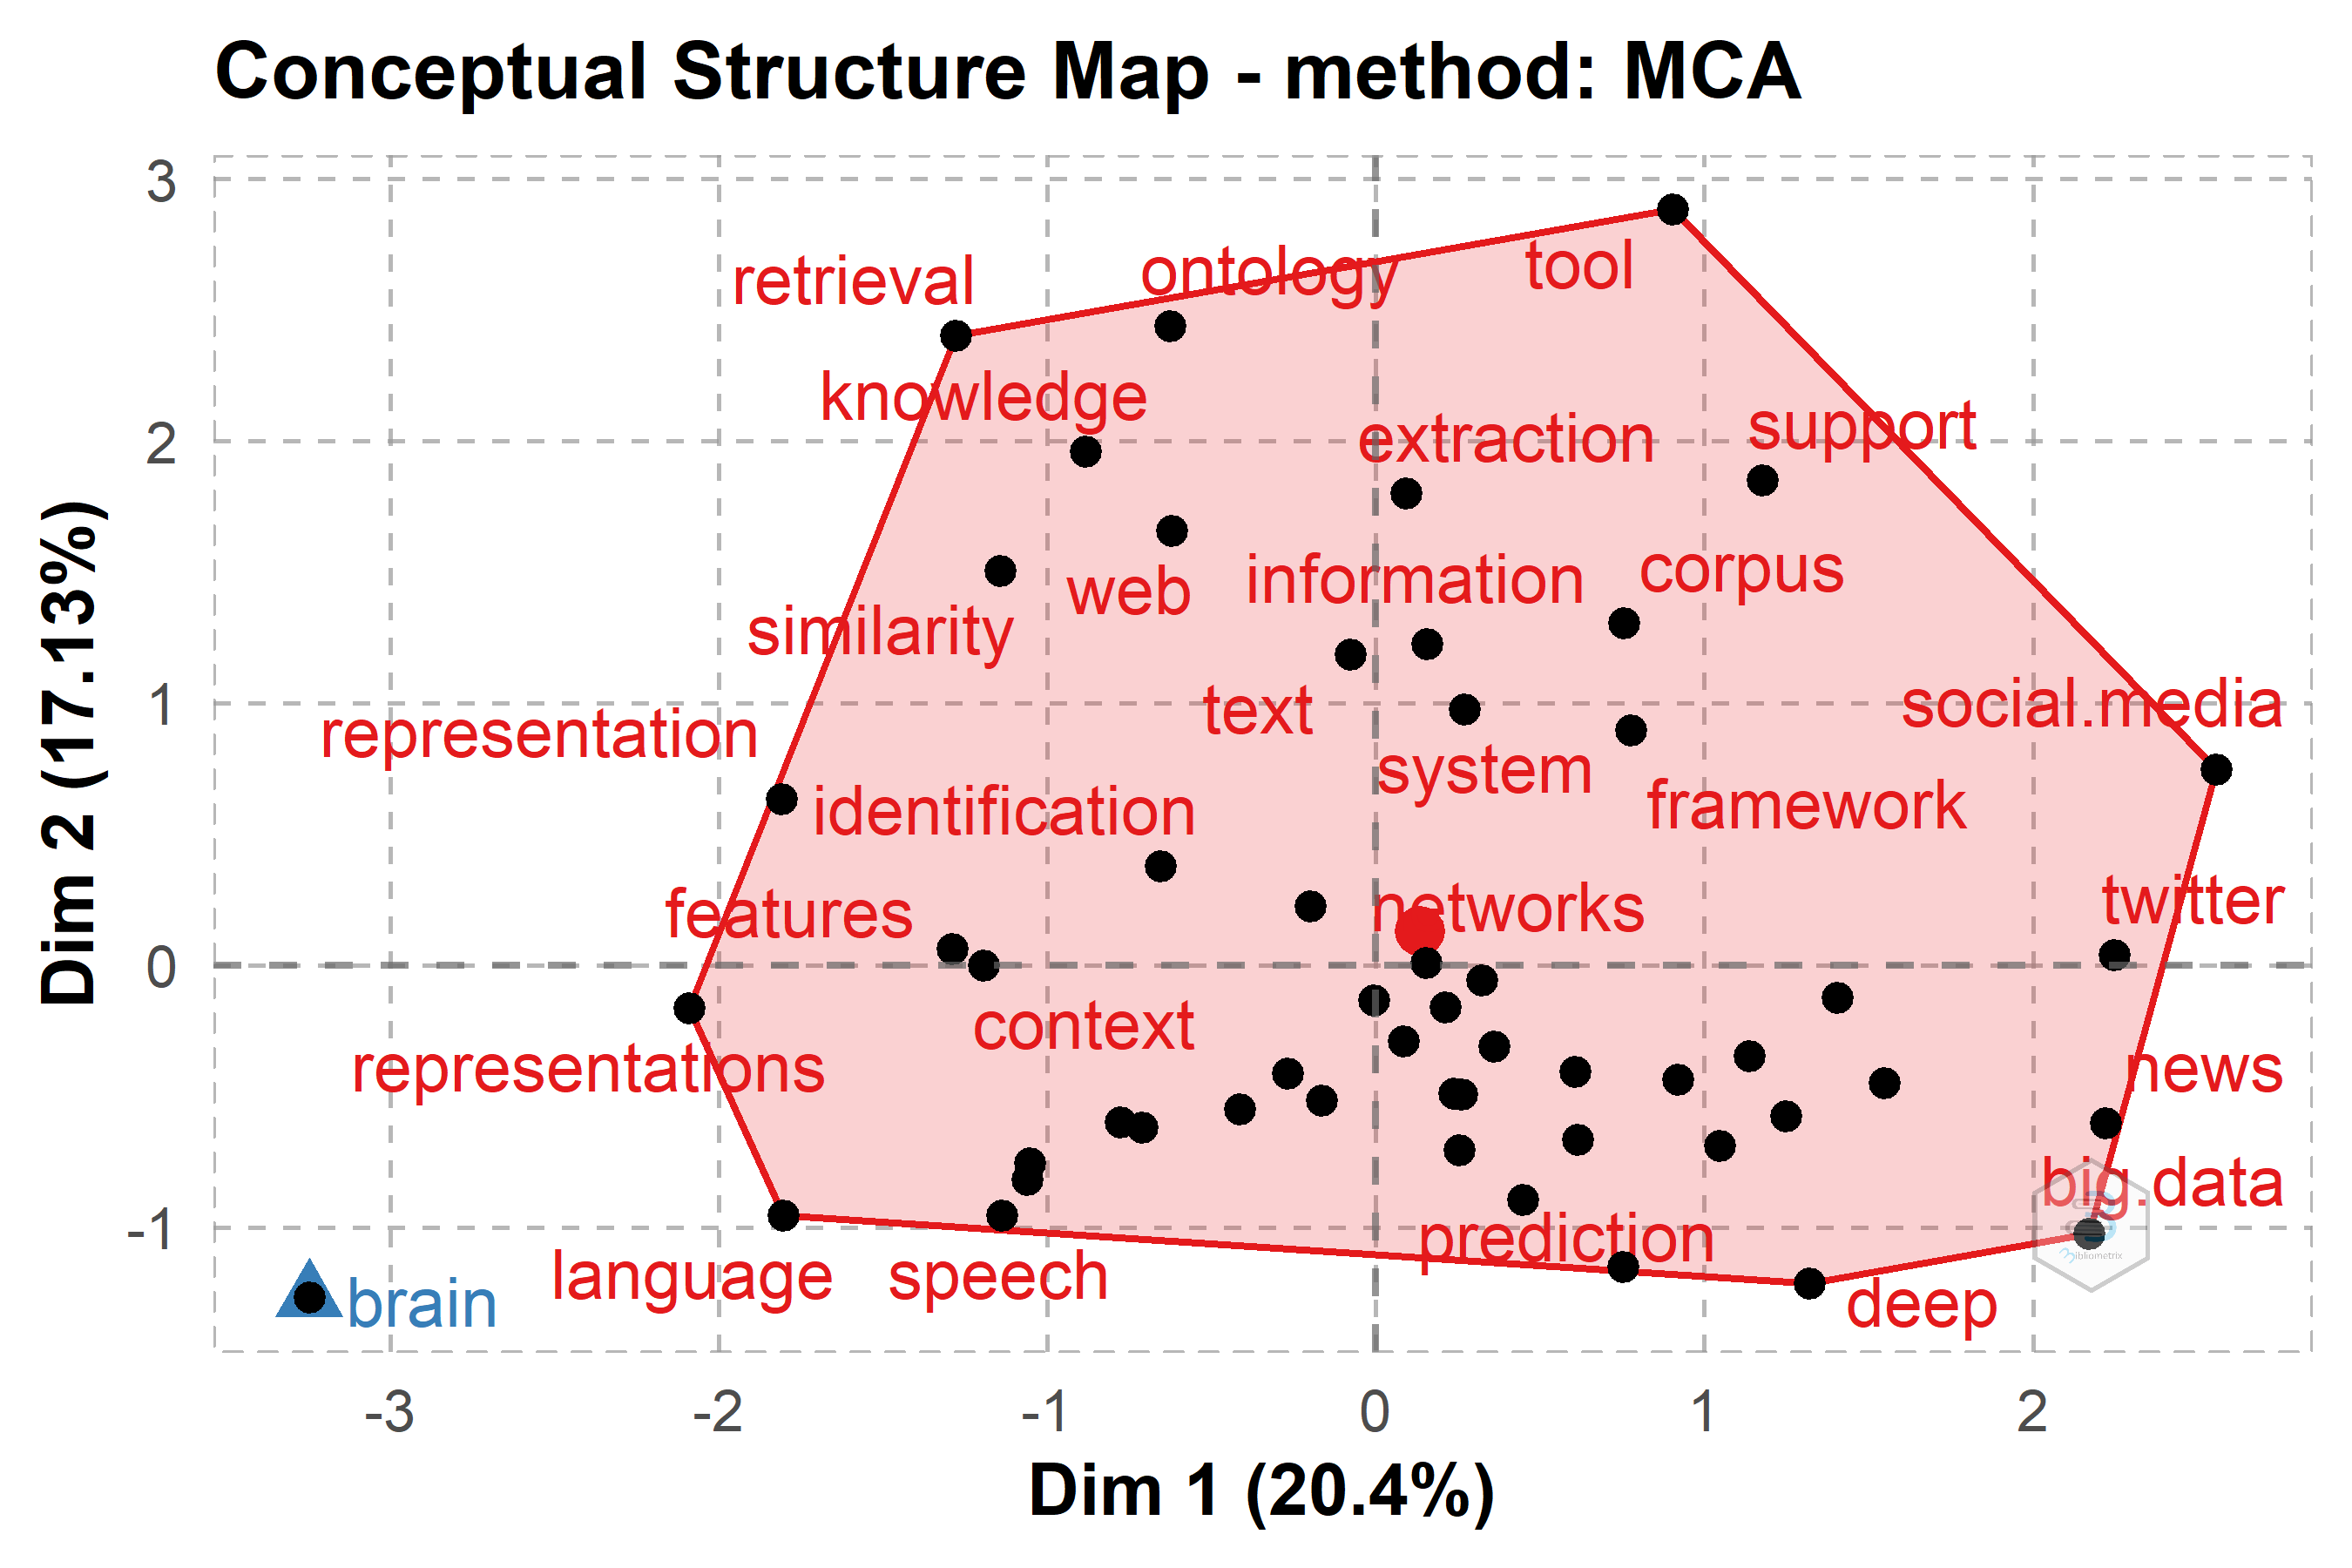
\includegraphics[width=1\textwidth]{experiments/ABMHub/PesquisaBibliometrica/NLP/estruturaConceitual.png}
    \caption{Estrutura conceitual do dataset\textit{NLP2@LABM}}
    \label{fig:ABMHub:EC}
\end{figure}

Podemos observar que há uma grande correlação entre todos os tópicos presentes no dataset. Era de se esperar, pois NLP está intrinsecamente e igualmente ligado com com conceitos como extração (de dados), deep learning, fala, linguagem, conhecimento, etc. Todos esses conceitos caminham juntos quando o assunto é NLP, pois todos eles compõem ou são produtos de NLP.

Mas existe um ponto no canto inferior esquerdo, em um agrupamento separado do agrupamento principal, com a label "brain". Um único tópico é pouco para definir o que exatamente esse ponto representa, portanto, é necessário forçar mais pontos no mapa para tentar traçar um padrão.

 \begin{figure}
    \centering
    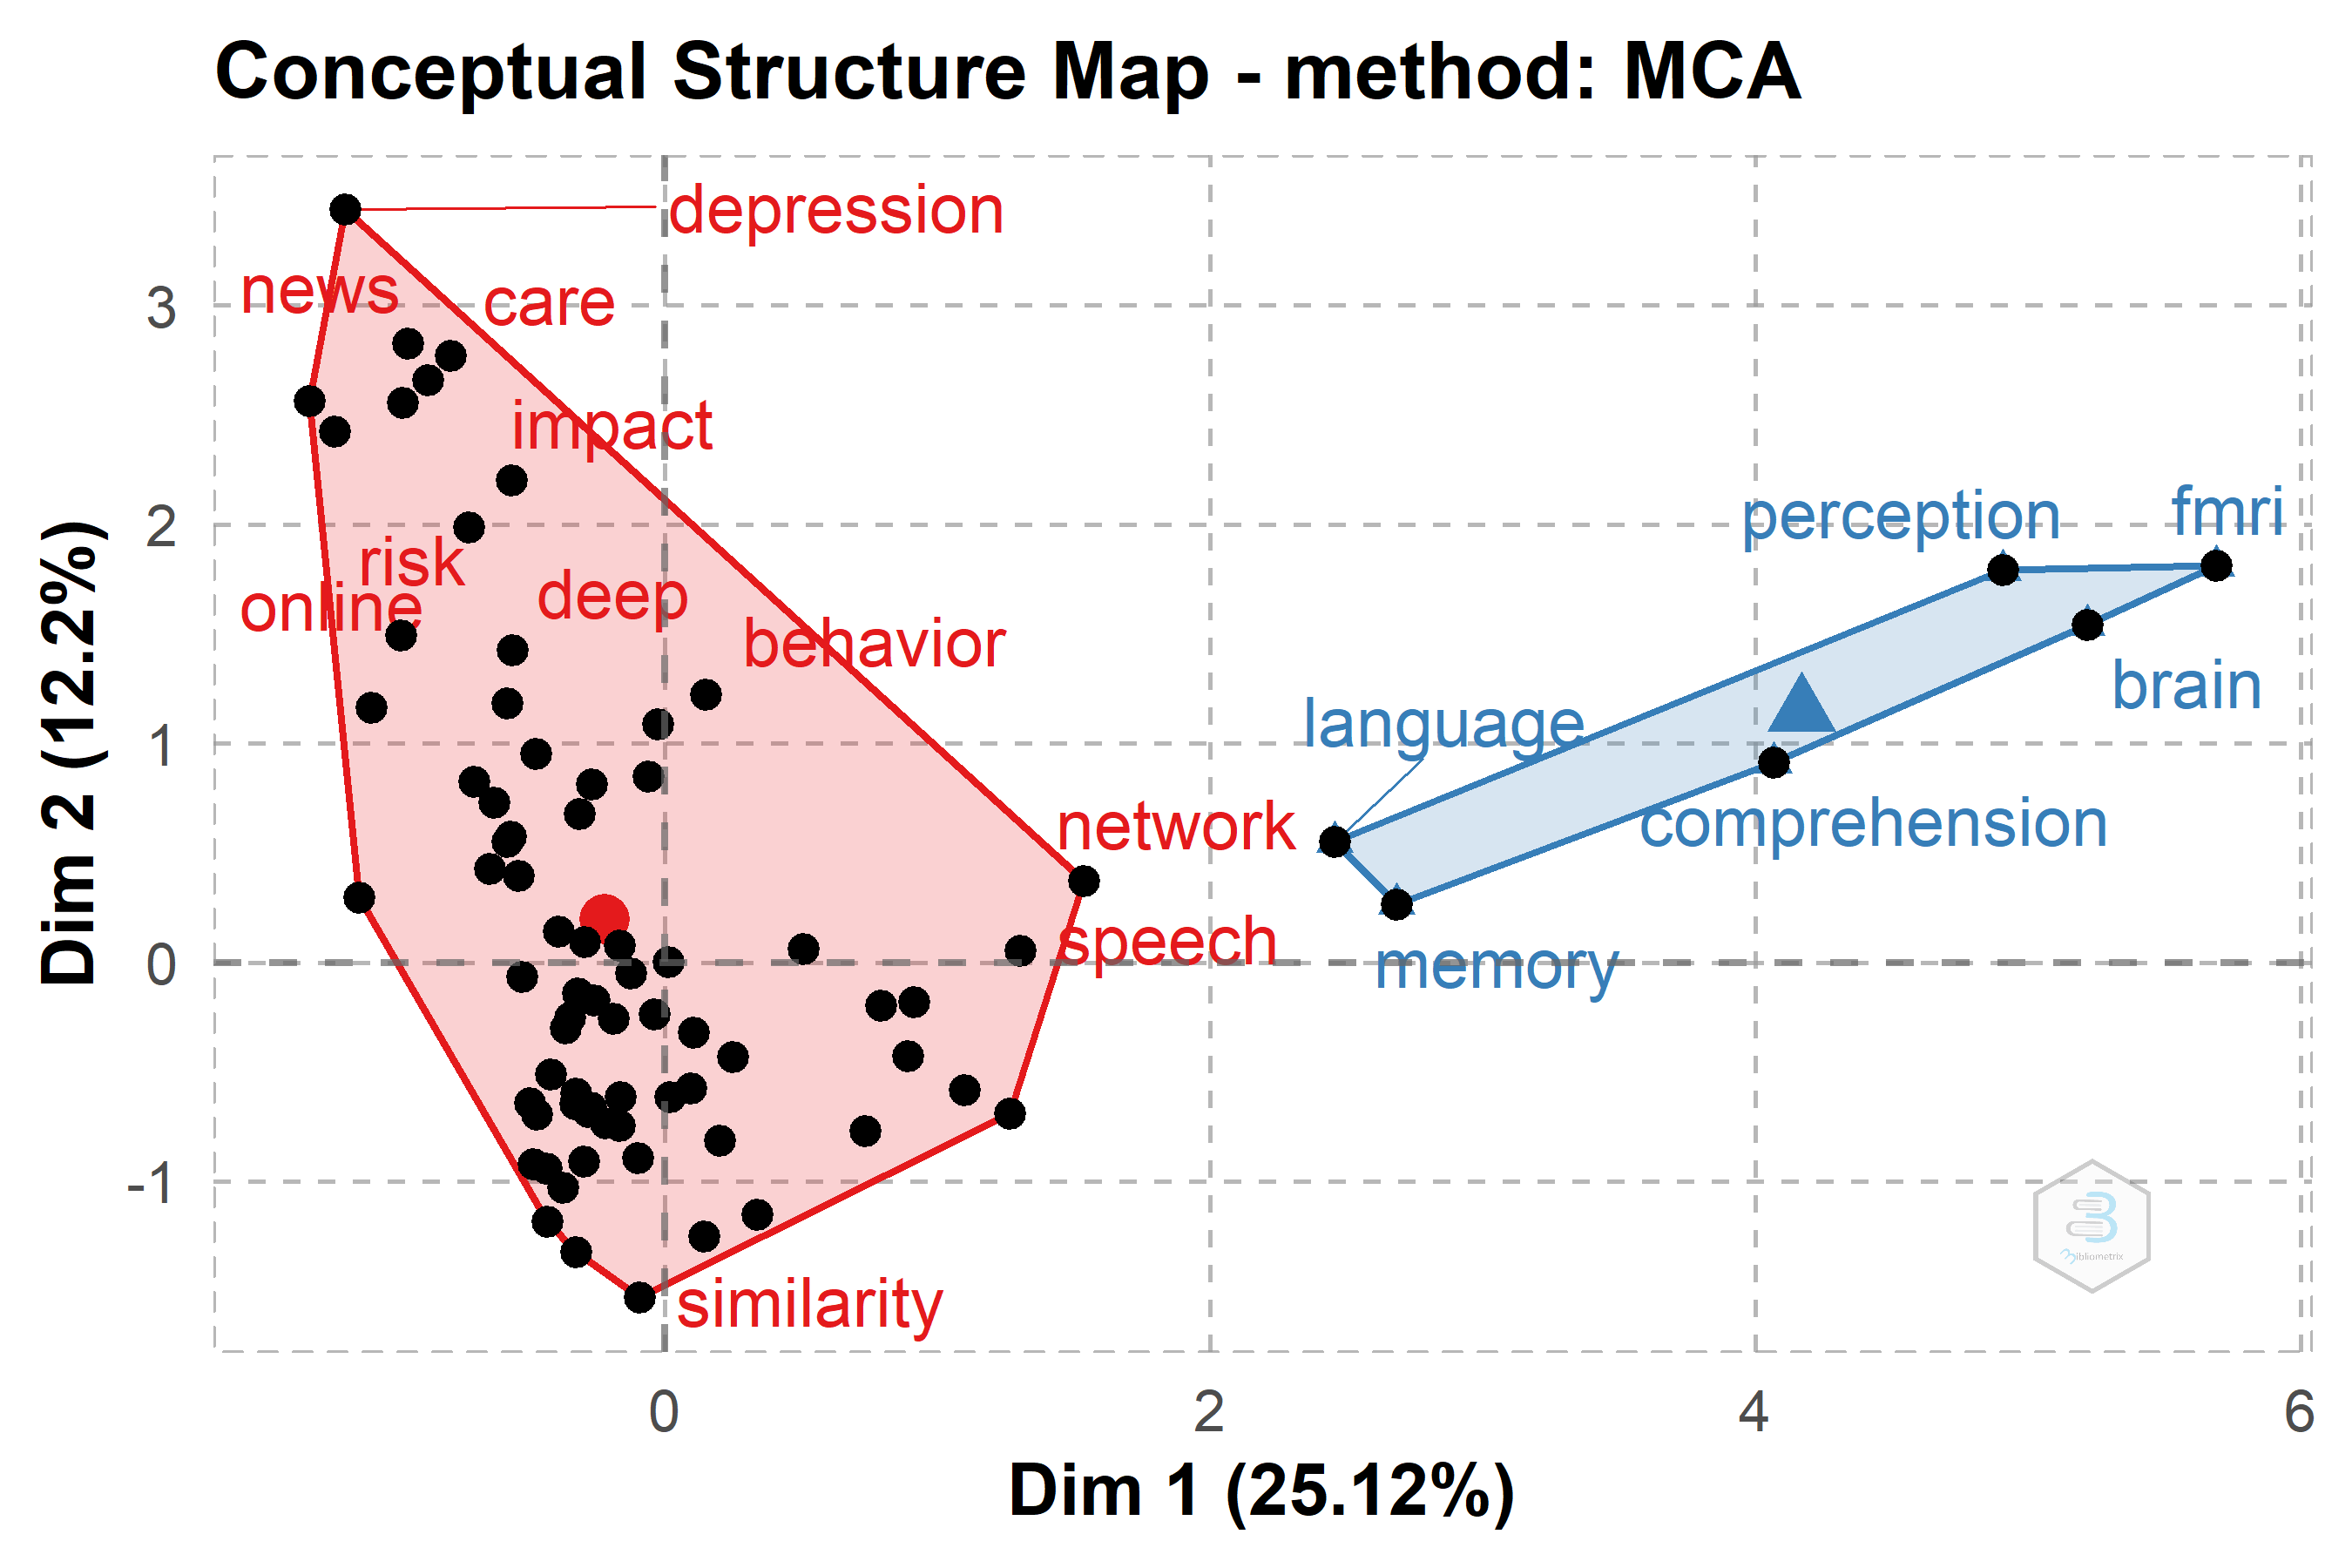
\includegraphics[width=1\textwidth]{experiments/ABMHub/PesquisaBibliometrica/NLP/estruturaConceitual2.png}
    \caption{Estrutura conceitual com 100 nós do dataset\textit{NLP2@LABM}}
    \label{fig:ABMHub:EC2}
\end{figure}

Conseguimos ver, na figura \ref{fig:ABMHub:EC2}, o que aquele ponto representava: um cluster de estudos da mente. Tópicos como memória, compreensão, cérebro, percepção, linguagem, etc, podem representar duas vertentes: estudiosos que tentam usar ferramentas de deep learning para progredir nos estudos da mente (afinal, redes neurais são inspiradas no comportamento do cérebro), e estudiosos que usam os conhecimentos da mente para progredir nos estudos de deep learning (pelo mesmo motivo que o anterior). Em ambos os casos, é interessante ver esse cluster no dataset.

\subsection{Análise da estrutura social}

A última pergunta que devemos responder, e ainda não foi respondida, é sobre a estrutura social da comunidade de NLP. Para isso, daremos uma olhada na rede de colaborações do dataset \textit{NLP2@LABM}, relacionando os países entre si (figura \ref{fig:ABMHub:social}).

\begin{figure}
    \centering
    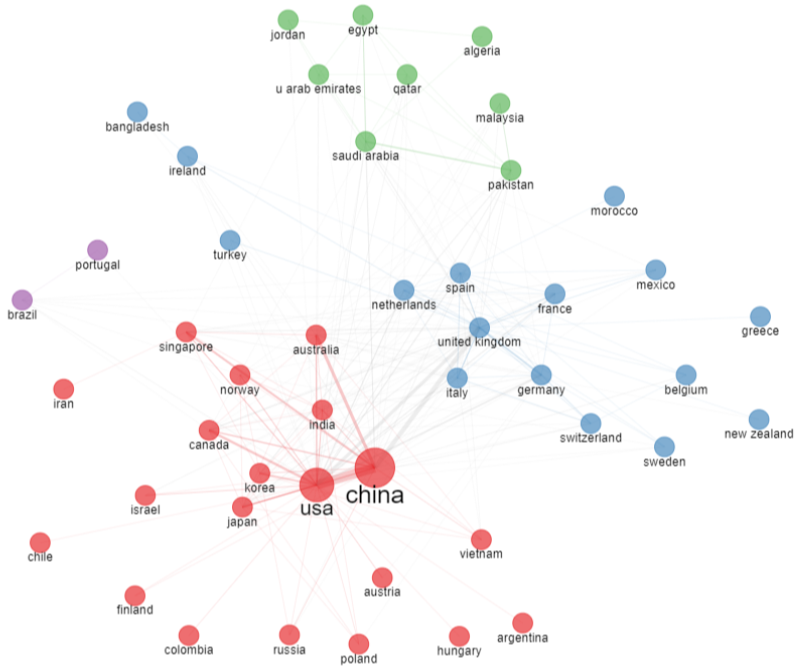
\includegraphics[width=1\textwidth]{experiments/ABMHub/PesquisaBibliometrica/NLP/socialStructure.png}
    \caption{Estrutura social de países do dataset\textit{NLP2@LABM}}
    \label{fig:ABMHub:social}
\end{figure}

Podemos ver, imediatamente, que as duas grandes potencias da área são Estados Unidos e China. Isso já era esperado, pois são as duas maiores potencias da ciência, como um todo. Nesse mesmo cluster, conseguimos encontrar outros países desenvolvidos, como Japão e Canadá, que costumam também ser grandes contribuintes para a ciência mundial. O cluster em azul, por outro lado, já apresenta uma reunião de países majoritariamente europeus, com algumas exceções de países emergentes, como Brasil e Rússia. Finalmente, o último cluster da imagem apresenta países majoritariamente do oriente médio, e contêm menos ligações que os outros dois clusters.

Com essa dominância absoluta da China e dos Estados Unidos sobre os outros países, fica a pergunta: como essa divisão de conhecimento é feita internamente no país? O grafo da figura \ref{fig:ABMHub:social2} responde essa pergunta.

\begin{figure}
    \centering
    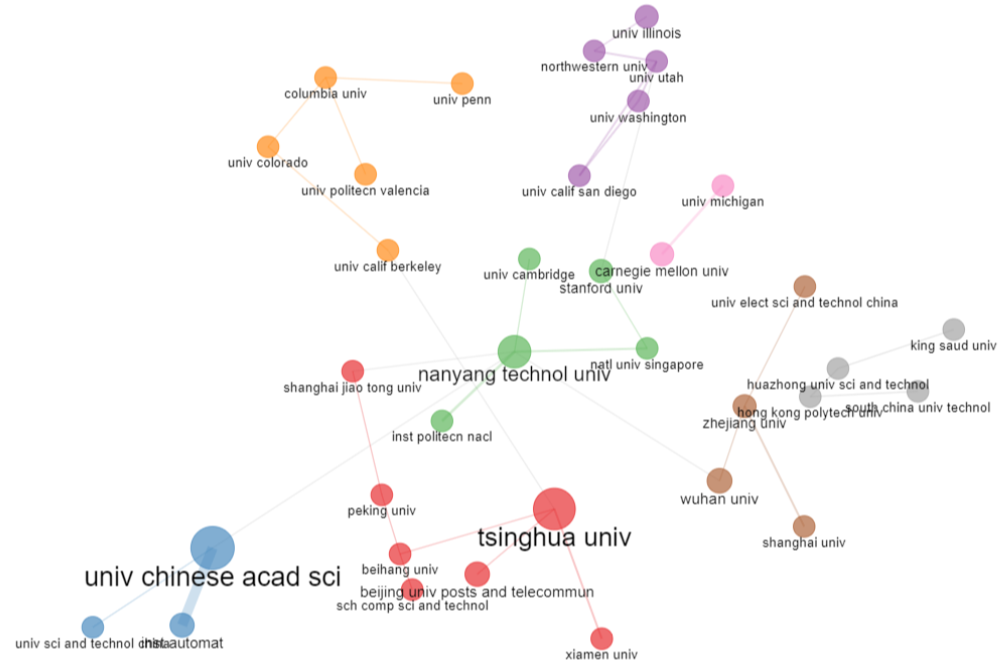
\includegraphics[width=1\textwidth]{experiments/ABMHub/PesquisaBibliometrica/NLP/socialStructure2.png}
    \caption{Estrutura social de universidades do dataset\textit{NLP2@LABM}}
    \label{fig:ABMHub:social2}
\end{figure}

Podemos ver que há, na China, uma concentração muito alta de conhecimento em uma pequena quantidade de universidades. Seguindo o sentido contrário, nos Estados Unidos, o conhecimento é muito mais diluído entre várias universidades diferentes. O interessante desses dois países é que, como visto na figura \ref{fig:ABMHub:social}, os dois países apresentam uma quantidade quase igual de artigos publicados, mas a divisão de conhecimento interno aos países é absolutamente diferente.

Uma última análise no quesito social é descer mais um nível e olhar o grafo de relação entre diferentes autores (figura \ref{fig:ABMHub:social3}).

\begin{figure}
    \centering
    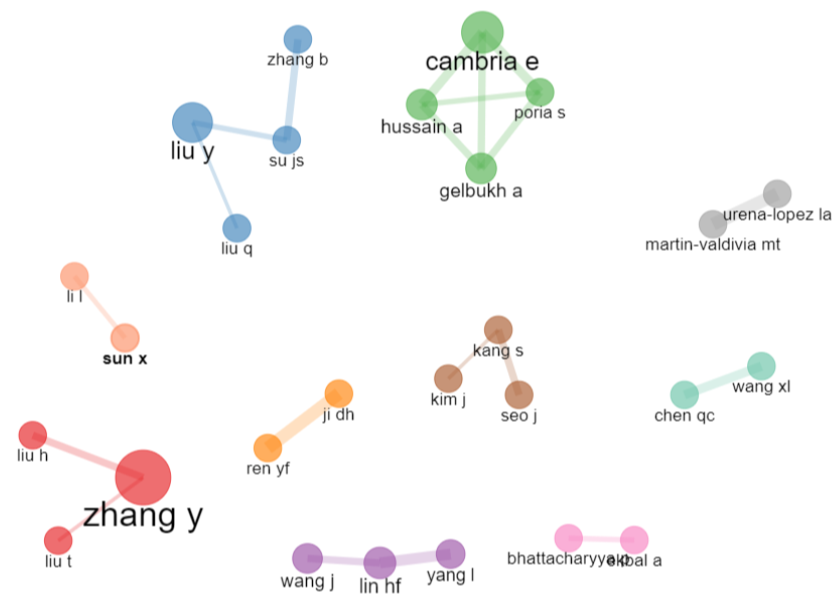
\includegraphics[width=1\textwidth]{experiments/ABMHub/PesquisaBibliometrica/NLP/socialStructure3.png}
    \caption{Estrutura social entre autores do dataset\textit{NLP2@LABM}}
    \label{fig:ABMHub:social3}
\end{figure}

Podemos observar, de imediato, a grande quantidade de estudiosos chineses, e seus grupos com muito impacto na área. Mais da metade dos clusters, e os com maior impacto, são de autores chineses. Porém, o cluster composto de Soujanya Poria, Amir Hussain, Erik Cambria e Alexander Gelbukh é uma exceção a regra. Esses autores são de Singapura, e os 4 têm um impacto muito grande nesse grafo, com vários trabalhos, a maioria com os quatro em grupo.